% !TeX root = main.tex
\section{The Maslov Index}

\subsection{The General Definition}

Let $H$ be a periodic Hamiltonian with flow $\phi_t$. The Maslov index is an integer associated to a nondegenerate contractible $T$-periodic orbit $\gamma$. The process is involved, but the process is roughly the following.
\begin{enumerate}[algorithm]\label{page:maslovalg}
\item\label{maslovalg:step1} Since $\gamma$ is periodic, it may be seen as a smooth map $S^1 \to M$.
\item Pick an embedding of the disk $D^2 \to M$ whose restriction to the border coincides with $\gamma$.
\item Pick smooth functions $Z_1(x), \dots, Z_{2n}(x) \colon D^2 \to TM$, such that $\{Z_i(x)\}$ forms a symplectic basis for $T_x M$.
\item Now that $T_{\gamma(t)} M$ has a chosen basis for each $t$, we may write the derivative of the flow at $x$, i.e. the map $(\dl \phi_t)_x$, as a $2n \times 2n$ symplectic matrix, which we will call $A(t)$. Note that $A(t)$ will not be periodic.
\item\label{maslovalg:step5} Given a path of symplectic matrices, such as $A(t)$, where $A(T)$ has no eigenvalue equal to one, it is possible to associate to it an integer called the Conley-Zehnder index.
\end{enumerate}

In turn, it is now necessary to compute the Conley-Zehnder index of a path of matrices $A(t)$. To do so first requires one to establish the existence of a map from the symplectic matrices to $S^1$.

\begin{theorem}\label{rhodef}
There exists a unique map $\rho \colon Sp(2n) \to S^1$ which satisfies the following properties.
\begin{enumerate}[label=\roman*)]
\item If $A$ and $T$ are symplectic matrices, $\rho(T A T^{-1}) = \rho(A)$,
\item If $A$ and $B$ are symplectic matrices,
\begin{equation}
\rho\left(\begin{bmatrix} A & 0 \\ 0 & B \end{bmatrix}\right) = \rho(A) \rho(B),
\end{equation}
\item\label{rhodef:xy} If $A$ is a symplectic matrix of the form $A = \begin{bmatrix} X & -Y \\ Y & X \end{bmatrix}$ then
\begin{equation}
\rho(A) = \det(X + \I Y).
\end{equation}
\item\label{rhodef:realev} If all eigenvalues of $A$ are real, then
\begin{equation}
\rho(A) = (-1)^{m_0/2},
\end{equation}
where $m_0$ is the number of negative eigenvalues, counted with multiplicity,
\item $\rho(A^\transposed) = \rho(A^{-1}) = \conj{\rho(A)}$.
\end{enumerate}

Furthermore, if $A$ is a symplectic matrix whose eigenvalues are all distinct, $\rho(A)$ may be computed using the following formula
\begin{equation}\label{rhoformula}
\rho(A) = (-1)^{m_0/2} \prod \lambda^{\sign \Im \omega(\conj v, v)},
\end{equation}
where the product is taken over the eigenvalues of $A$ with positive imaginary part and unit norm, and to each such $\lambda$ we have associated  a (in general, complex) eigenvector $v$, and we have implicitly extended the 2-form $\omega$ on $\R^{2n}$ in the obvious way to $\C^{2n}$.
\end{theorem}

\begin{proof}
See \cite{audin}, Theorem 7.1.3 on page 192.
\end{proof}

We are now ready to define the Maslov index of a path of symplectic matrices $A(t)$:

\begin{enumerate}[algorithm]
\item Define $Sp(2n)^*$ as the collection of symplectic matrices that do not have 1 as an eigenvalue. It is a known fact \cite[proposition~7.1.4]{audin} that $Sp(2n)^*$ is composed of two path-connected components, $Sp(2n)^+$ and $Sp(2n)^-$, labeled by the sign of $\det(A-I)$. Note that $A(T) \in Sp(2n)^*$, so it must lie in one of these two components.
\item\label{maslov:step2} Define the matrices $W^+$ and $W^-$ as
\begin{equation}
W^+ = - I, \quad W^- \mleft[\begin{array}{c|c}
\begin{matrix} 2 & 0 \\ 0 & 1/2 \end{matrix} & 0\\
\hline
0 & -I
\end{array}\mright].
\end{equation}
Note that $W^\pm \in Sp(2n)^\pm$, and so any matrix in $Sp(2n)^*$ can be connected via a path (in $Sp(2n)^*$) to either $W^+$ or $W^-$. Consequently, we extend $A(t)$ to the interval $\interval 0 {2T}$, where for $t \in \interval T {2T}$ the path $A(t)$ represents such a path connecting $A(2T)$ to $W^\pm$.
\item Define $\alpha(t) = \rho(A(t))$ for $a \in \interval 0 {2T}$. It is trivial to check using property \ref{rhodef:realev} from theorem \ref{rhodef} that $\rho(W^\pm) = (-1)^n$, and also that $\rho(I) = 1$. Therefore, $\rho \circ \alpha$ is a path in $S^1$ starting at $1$ and ending at $1$ or $-1$. Therefore, taking the square (viewing $S^1 \subseteq \C$) one obtains a loop $\rho^2 \circ \alpha$ starting and ending at $1$.
\item Now that we have a loop in $S^1$, we can obtain an integer by considering its winding number: the number of times the loop does a full turn around the circle. It is necessary to establish which direction is positive. Generally, one considers the counterclockwise direction to be the positive direction, but for purposes of the Conley-Zehnder index we count the number of \emph{clockwise turns}.
\end{enumerate}
The resulting number of the above procedure is called the Conley-Zehnder index of $A$, denoted $\mu(A)$, and finally we define the Maslov index of the periodic orbit $\gamma$ above, also denoted with the symbol $\mu(\gamma)$, as the Conley-Zehnder index of the corresponding matrix path $A$.

It is a very nontrivial fact that the corresponding integer does not depend on any of the choices done in the process, only on the path and on the Hamiltonian flow. The details may be found in \cite{audin}, whose whole 7th chapter is dedicated to the definition, and well-definition, of this index.

\subsection{The Particular Case of $Sp(2)$}\label{sec:maslovsp2}

The theory of the Maslov index simplifies greatly in the two-dimensional case. This is partly due to the much greater control over the spectrum of a matrix. In two dimensions, the symplectic matrices coincide with those whose determinant equals one, and so their spectrum is entirely determined by their trace.

\begin{prop}
Let $A = \mleft[\begin{smallmatrix} a & b \\ c & d \end{smallmatrix}\mright]$ be a $2 \times 2$ symplectic matrix, that is, it satisfies the equation $ad - bc = 1$. Then, the spectrum of $A$ can be written in terms of its trace, $\tau = a+d$, as
\begin{equation}\label{lambdafromtau}
\lambda_\pm = \frac{\tau \pm \sqrt{\tau^2 - 4}}2.
\end{equation}

Consequently, the behavior of the spectrum can be qualitatively described as follows
\begin{itemize}
\item If $\tau \geq 2$, both eigenvalues are positive real numbers,
\item If $-2 \leq \tau \leq 2$, both eigenvalues lie on the unit circle as a conjugate pair,
\item If $\tau \leq -2$, both eigenvalues are negative real numbers.
\end{itemize}
\end{prop}

\begin{proof}
Equation \eqref{lambdafromtau} is a trivial consequence of the fact that the characteristic polynomial of a $2 \times 2$ matrix $A$ is $p(\lambda) = \lambda^2 - (\trace A) \lambda + \det A$.

The quantitative behavior is proved in two cases.
\begin{itemize}
\item Suppose that $\abs \tau \geq 2$. Then, it is easy to check that $\lambda_\pm$ is real. Furthermore, $\lambda_{\sign \tau}$ clearly has the same sign as $\tau$, and since $\lambda_+ \lambda_- = 1$, both eigenvalues must have the same sign.
\item Suppose that $\abs \tau \leq 2$. Then, the square root term is purely imaginary and so the absolute value of $\lambda_\pm$ can be easily computed by the pythagorean theorem. Since the norm of $\lambda_\pm$ equals one and $\lambda_+ = 1/\lambda_-$, it is trivial to conclude that $\lambda_+ = \conj{\lambda_-}$.
\end{itemize}
\end{proof}

\begin{corollary}\label{sp2sgn}
A matrix $A \in Sp(2)$ is in $Sp(2)^*$ iff $\trace A \neq 2$. In this case, it is in $Sp(2)^{\sign(2 - \trace A)}$.
\end{corollary}

\begin{proof}
Using the notation of proposition \ref{lambdafromtau}, since $\lambda_+ \lambda_- = 1$, the only way for either eigenvalue to be equal to 1 is for both of them to be equal to 1. Therefore, if any eigenvalue is one, $\trace A = \lambda_+ + \lambda_- = 2$. On the other hand, if $\trace A = 2$ it is obvious that both eigenvalues are one.

To determine the sign of $\det(A-I)$, we compute it directly as
\begin{equation}
\det(A-I) = p(1) = 1^2 - (\trace A) \times 1 + \det A = 2 - \trace A.
\end{equation}
\end{proof}

\begin{remark}
Note the counter-intuitive signs. If $\trace A > 2$ then $A \in Sp(2)^-$, not $Sp(2)^+$. The counter-intuitiveness extends to the $W^\pm$ matrices, given the regrettable fact that $\rho(W^\pm) = \mp 1$.
\end{remark}

\begin{corollary}\label{sp2pm}
Let $A \in Sp(2)$. Then, $\rho(A) = 1$ iff $A \in Sp(2) \setminus Sp(2)^+$, i.e. iff $\trace A \geq 2$. Furthermore, $\rho(A) = -1$ iff $\trace A \leq -2$.
\end{corollary}

\begin{proof}
We divide the proof in three cases.
\begin{itemize}
\item If $\trace A \geq 2$, both eigenvalues of $A$ are positive, and so using property \ref{rhodef:realev} from theorem \ref{rhodef} one concludes $\rho(A) = 1$.
\item If $\trace A \leq -2$, both eigenvalues of $A$ are negative, and so for the same reason $\rho(A) = -1$.
\item If $-2 < \trace A < 2$, both eigenvalues are in $S^1 \setminus \R$. Furthermore, they are both distinct, and so we may apply equation \eqref{rhoformula} to compute
\begin{equation}\label{sp2pm:3}
\rho(A) = \lambda_+^\sigma,
\end{equation}
where $\sigma$ is either $1$ or $-1$. Therefore, in this case $\rho(A)$ is either $\lambda_+$ or $\lambda_-$ and necessarily not a real number.
\end{itemize}
\end{proof}

The above propositions, notably corollary \ref{sp2pm}, greatly simplify the work of calculating the Maslov index in dimension 2, specifically in step \ref{maslov:step2}, which consists of extending the path $A(t)$ to one with endpoint in $W^\pm$.

\begin{corollary}\label{sp2rhoextension}
Let $A \in Sp(2)^*$, and define $A(t)$ as a path in $Sp(2)^*$ such that $A(0) = A$ and $A(1) = W^\pm$. Then, $\rho(A(t))$ has one of two possible behaviors:
\begin{itemize}
\item If $\rho(A) = 1$ then $\rho(A(t))$ is constant equal to one,
\item If $\rho(A) \neq 1$ then $\rho(A(t))$ is a path in $S^1 \setminus \{1\}$ with $\rho(A(1)) = -1$.
\end{itemize}
\end{corollary}

\begin{proof}
If $\rho(A) = 1$ then $A \in Sp(2)^-$ by corollary \ref{sp2pm}. Since the path connecting $A$ to $W^-$ remains in $Sp(2)^-$, and so $\rho(A(t))$ is constant equal to 1 by the same corollary.

If $\rho(A) \neq 1$ then $A \in Sp(2)^+$, and so $A(t)$ connects $A$ to $W^+$. Since this path does not leave $Sp(2)^+$ it never attains the value $1$, and $\rho(A(1)) = \rho(W^+) = -1$.
\end{proof}

Due to corollary \ref{sp2rhoextension}, the algorithm to calculate the Maslov index of a path of matrices can be simplified as follows.

\begin{prop}
Let $A(t)$ be a path of matrices in $Sp(2)$ with $A(T)$ in $Sp(2)^*$. Then, the Maslov index of the path $A(t)$ can be computed as follows:

\begin{enumerate}[algorithm]
\item Compute the path $\gamma(t) = \rho(A(t))$. 
\item If $\gamma(1) \neq 1$, extend it by connecting $\gamma(1)$ to $-1$, without passing through 1, otherwise leave it as-is. Call the resulting curve $\gamma_0$.
\item Compute the (clockwise) winding number of $\gamma_0^2$.
\end{enumerate}
\end{prop}

To conclude this section, we present a further way to simplify the computations. The essential observations are the following.
\begin{itemize}
\item It is trivial to compute $\rho(A)$ when $\abs{\trace A} \geq 2$, as it coincides with $\sign A$,
\item $\rho(A)$ is never $\pm 1$ when $\abs{\trace A} < 2$,
\item We are only interested in the winding number of $\rho^2(A(t))$,
\item And consequently, if for some $t_0, t_1$ we have $\trace A(t_0) = - \trace A(t_1) = \pm 2$ and $-2 < \trace A(t) < 2$ for $t_0 < t < t_1$, it suffices to compute $\rho(A(t))$ for a sigle value of $t \in \ointerval{t_0}{t_1}$.
\end{itemize}

\begin{prop}\label{calcmaslov}
Let $A(t)$, $t \in \interval 0 T$ be a path of matrices with $A(0) = I$, $A(T) = W^\pm$. If $\trace A(t) \geq -2$ for all time, the Maslov index of $A$ is zero. Otherwise, there exists a partition of $\interval 0 T$ of the form
\begin{equation}\label{calcmaslov:ab1}
0 = a_0 < b_0 < a_1 < b_1 < a_2 < \dots < a_{N-1} < b_{N-1} < a_N = T
\end{equation}
which satisfies the properties
\begin{enumerate}
\item\label{calcmaslov:ab2} $(-1)^n \trace A(a_n) \geq 2$, \item\label{calcmaslov:ab3} $\trace A(b_n) = 0$, \item\label{calcmaslov:ab4} Whenever $\trace A(x) \geq 2$ and $\trace A(y) \leq -2$, there exists some $b_n$ between $x$ and $y$.\end{enumerate}

For any such partition, the negative winding number of $\rho^2(A(t))$ is equal to
\begin{equation}\label{calcmaslov:mu}
\mu(A(t)) = \sum (-1)^n \sign(A(b_n)_{12}).
\end{equation}
\end{prop}

\begin{proof}
First we do the easy part: If $\trace A(t) > -2$ for all time, the Maslov index of $A(t)$ is null.

By corollary \ref{sp2pm}, this hypothesis implies that $\rho(A(t))$ is never $-1$. Consequently, the path $\rho(A(t))$ is contractible, and therefore so is $\rho^2(A(t))$. As such, the winding number of $\rho^2(A(t))$ is zero, and so is the Maslov index.

Now, assume that $\trace A(t) \leq -2$ for some $t$. We prove that a partition \eqref{calcmaslov:ab1} satisfying \ref{calcmaslov:ab2}, \ref{calcmaslov:ab3} and \ref{calcmaslov:ab4} exists.

Let $U \subseteq \interval 0 T$ be the preimage under $\trace \circ A$ of $\ointerval{-2}\infty$, and $V$ the preimage of $\ointerval{-\infty}2$. Then, by standard Lebesgue number lemma arguments, there exists a partition 
\begin{equation}
0 = c_0 < c_1 < \dots < c_{N+1} = T,
\end{equation}
such that each interval $\interval{c_n}{c_{n+1}}$ is entirely contained in $U$ or $V$. By removing unnecessary partitions, we may suppose without loss of generality that
\begin{equation}
\interval{c_0}{c_1} \subseteq U, \interval{c_1}{c_2} \subseteq V, \interval{c_2}{c_3} \subseteq U, \dots,
\end{equation}
and furthermore that for each $n$ there exists some $t_n \in \ointerval{c_n}{c_{n+1}}$ such that $t_n \in U \setminus V$ or $t_n \in V \setminus U$. Without loss of generality pick $t_0 = c_0 = 0$ and $t_N = c_{N+1} = T$. (In this step, we are assuming that $0 \neq N$, which is why the case $\forall_t \trace A(t) > -2$ must be done separately.)

We now have a sequence of numbers
\begin{equation}\label{tcineq}
0 = t_0 < c_1 < t_1 < c_2 < t_2 < \dots < t_{N-1} < c_{N-1} < t_{N} = T.
\end{equation}

We will now perturb this sequence, in order to obtain the $a_n$ from the $t_n$ and the $b_n$ from the $c_n$.

Note that $\trace A(t_0) = 2$, $\trace(A(t_1)) \leq -2$, $\trace(A(t_2)) \geq 2$, and so on. By continuity, we may assume without loss of generality that these inequalities are equalities, and since $\trace(A(c_i)) \in \ointerval{-2}2$ we may assume that the inequalities \eqref{tcineq} still hold.

The resulting sequence $t_0, t_1, \dots$ is renamed to $a_0, a_1, \dots$, and we now turn to constructing the sequence $b_1, b_1, \dots$

By compacity, between each $a_n, a_{n+1}$ there exists a maximal $\alpha_n$ satisfying $\trace A(\alpha_n) = \trace A(a_n)$ and a minimal $\alpha'_{n+1}$ with $\trace A(\alpha'_{n+1}) = \trace A(a_{n+1})$. It is easy to check the inequalities
\begin{equation}
a_n \leq \alpha_n < c_n <\alpha'_{n+1} \leq a_{n+1},
\end{equation}
and therefore by continuity there exists some $b_n$ satisfying
\begin{equation}
\trace A(b_n) = 0, \quad \alpha_n < b_n < \alpha'_{n+1}.
\end{equation}

It is obvious that the inequalities \eqref{calcmaslov:ab1} hold, as well as properties \ref{calcmaslov:ab2} and \ref{calcmaslov:ab3}. It remains to prove property \ref{calcmaslov:ab4}, i.e., that whenever $\trace A(x) \geq 2$ and $\trace A(y) \leq -2$ there exists some $b_n$ between $x$ and $y$.

To prove property \ref{calcmaslov:ab4}, we make the following remark.
\begin{lemma}\label{calcmaslov:lemma1}
The sequence of intervals $\interval 0 {b_0}, \interval {b_0}{b_1}, \interval{b_1}{b_2}, \dots, \interval{b_{N-1}}T$ is alternatively contained in $U$ and in $V$.
\end{lemma}

\begin{lemmaproof}
The proof of lemma \ref{calcmaslov:lemma1} is a simple but laborious application of the maximalities and minimalities of the $\alpha_n$ and $\alpha'_n$. As an example, we will prove that $\interval{b_0}{b_1} \subseteq V$.

Suppose that $\trace A(t) \geq 2$ for some $t \in \interval{b_0}{b_1}$. By continuity, we may suppose without loss of generality that $\trace A(t) = 2$. Then, it is the case that either $t \in \interval{a_0}{a_1}$ or $t \in \interval{a_1}{a_2}$. In the first case, by maximality of $\alpha_0$, we have
\begin{equation}
t < \alpha_0 < b_0 \leq t,
\end{equation}
an obvious contradiction. The case where $t \in \interval{a_1}{a_2}$ is done in a similar way, applying the minimality of $\alpha'_2$.
\end{lemmaproof}

The proof of property \ref{calcmaslov:ab4} is a simple consequence of the fact that, under the hypotheses of this property, $x \in U \setminus V$ and $y \in V \setminus U$. Therefore, $x$ and $y$ must be in distinct intervals among those in the statement of lemma \ref{calcmaslov:lemma1} and thus must be separated by at least one value of $b_n$.

\smallskip

We now turn to the last part of the proof: We suppose that we have a partition $(a_n, b_n)$ satisfying \eqref{calcmaslov:ab1} and properties \ref{calcmaslov:ab2}, \ref{calcmaslov:ab3} and \ref{calcmaslov:ab4} and we prove formula \eqref{calcmaslov:mu}.

First, observe that the winding number of $\rho^2(A(t))$ can be calculated in pieces, as the path $\rho^2 \circ A$ can be decomposed into its restriction to $\interval{a_0}{a_1}$, $\interval{a_1}{a_2}$, etc., so it suffices to calculate the winding number of $\rho^2(A(t))$ as $t$ varies from $a_n$ to $a_{n+1}$.

For the sake of argument, suppose that $n$ is even. We apply property \ref{calcmaslov:ab4} and corollary \ref{sp2pm} to observe that between $a_n$ and $b_n$ the trace of $A$ is never $-2$, and consequently $\rho(A(t))$ is never $-1$. Since $S^1 \setminus \{-1\}$ is contractible, there is a homotopy between every path from $\rho(A(a_n)) = 1$ and $\rho(A(b_n)) = \pm\I$.\footnote{It is an easy consequence of equation \eqref{sp2pm:3} from corollary \ref{sp2pm} that whenever a matrix $A$ has null trace, $\rho(A) = \pm \I$.} Therefore, without change to the winding number of $\rho^2$, we may replace the path $\rho(A(t))$ in $\interval{a_n}{b_n}$ by a reparametrization of $\pm \e^{\I \theta}$, $\theta \in \interval 0 {\pi/2}$. By the same argument, the path $\rho(A(t))$ for $t \in \interval{b_n}{a_{n+1}}$ may be replaced by $\pm \e^{\I \theta}$, $\theta \in \interval{\pi/2}\pi$, and so, for $t \in \interval{a_n}{a_{n+1}}$ the path $\rho^2(A(t))$ is homotopic to $\pm \e^{2 \I \theta}$, $\theta \in \interval 0 \pi$, with winding number $\pm 1$, where the sign is the sign of $\Im \rho(A(b_n))$.

If $n$ is odd, the previous argument works the same way, but the expression for the winding number of $\rho^2(A(t))$ has the sign swapped, i.e. it becomes $- \Im \rho(A(b_n))$. Therefore, we conclude the formula
\begin{equation}
\mu(A(t)) = -\sum (-1)^n \sign \Im \rho(A(b_n)).
\end{equation}

Note the sign swap from the definition of Maslov index. All that remains is to compute $\rho(A(b_n))$.

\begin{lemma}
Let $A$ be a $2 \times 2$ symplectic matrix with null trace. Then, $\rho(A) = -\sign(A_{12}) \cdot  \I$.
\end{lemma}

\begin{lemmaproof}
Let us name the entries of $A$. Suppose that
\begin{equation}
A = \begin{bmatrix}
a & b\\
c & d
\end{bmatrix}.
\end{equation}

Using the condition on the trace we obtain $d = -a$. Furthermore, the condition that $A$ is symplectic, i.e. its determinant is 1, yields
\begin{equation}
bc = -(1 + a^2),
\end{equation}
and since $a$ is real the right-hand side can never be null, therefore $b, c \neq 0$ and $c$ can be written in terms of $a$ and $b$, yielding
\begin{equation}
A = \begin{bmatrix}
a & b\\
-\frac{1+a^2}b & -a
\end{bmatrix}.
\end{equation}

To proceed, by equation \eqref{sp2pm:3} from corollary \ref{sp2pm}, $\rho(A) = \pm I$. Furthermore, this is true of any matrix $A$ with null trace, so if we continuously deform $A$ into some matrix $A'$ whose value of $\rho$ is well-known, without ever leaving the matrices with null trace, we $\rho(A) = \rho(A')$.

To begin, we continuously deform $b$ from its current value to $\pm 1$, without passing through zero. Then, we continuously deform $a$ into 0. At the end, we obtain the matrix
\begin{equation}
A' = \begin{bmatrix}
0 & \pm 1\\
\mp 1 & 0
\end{bmatrix},
\end{equation}
whose value of $\rho$ is known to be $\mp 1$ by property \ref{rhodef:xy} from theorem \ref{rhodef}. Since $\sign(b) = \pm 1$, we obtain the expected result
\begin{equation}
\rho(A) = - \sign(A_{12}).
\end{equation}
\end{lemmaproof}

This concludes the proof of the proposition.
\end{proof}

\subsection{The Autonomous Case}

Let $H$ be an autonomous Morse function on a symplectic manifold $M$ whose time-$T$ flow $\phi_T$ is a nondegenerate Hamiltonian diffeomorphism. In this section, we will compute the Maslov index of the critical points of $H$ and relate them to their Morse index. At the end, we will repeat the procedure for the two-dimensional case, as an example of application of the methods from section \ref{sec:maslovsp2}.

Let $x$ be a critical point of $H$, i.e. $(\dl H)_x = 0$. Then, the periodic time-$T$ orbit starting at $x$ is precisely the constant orbit. We will show that this orbit is nondegenerate, so that we may compute its Maslov index.
[...]

[Some theorem about in critical points $x$ of $H$, the path $A$ can be chosen to be $\exp(t J_0 S)$, where $S$ is the Hessian of $H$ at $x$ written in any basis.]

As a consequence, if $Z_1, \dots, Z_{2n}$ is a basis of $T_x M$, we may consider $A(t)$ as the representation of $(\dl \phi_t)_x$ in this basis (see steps \ref{maslovalg:step1} to \ref{maslovalg:step5}).

[Temporary? Kick the can up the road and just refer to Audin and Damian]

\begin{theorem}
If $S$ is an invertible symmetric matrix with operator norm $\norm S < \frac{2\pi}T$ and if $A(t) = \exp(t J_0 S)$, $t \in \interval 0 T$, then $A(T)$ is nondegenerate and
\begin{equation}
\mu(A(t)) = \Ind(S) - n,
\end{equation}
where $\Ind$ denotes the Morse index.
\end{theorem}

\begin{proof}
See \cite{audin}, proposition 7.2.1.
\end{proof}

\subsection{The Two-Dimensional Case}

We will now use the tools developed in section \ref{sec:maslovsp2} to recompute the Maslov index of the critical points of $H$.

[Nondegeneracy?]

We have already shown that the Maslov index of such a critical point is given by the Conley-Zehnder index of the path
\begin{equation}
A(t) = \exp(t J_0 S), t \in \interval 0 T,
\end{equation}
with $S = \hessian H(x)$, i.e. $S_{ij} = \hessian H(x)(Z_i, Z_j) = Z_i \cdot (Z_j \cdot H)$. It is therefore to such a path that we will focus our attention.

It is fortunate that the theory greatly simplifies in the two-dimensional case, allowing us to do the computations by hand.

\begin{prop}\label{prop:sidentities}
Let $S$ be a $2 \times 2$ symmetric matrix, and let $\Delta = \det S$. Then, the following identities hold.
\begin{gather}
J_0 S J_0 S = - \Delta I, \label{eq:j0sj0s}\\
\exp(t J_0 S) = \begin{cases}
\cos(\sqrt{\Delta} t) I + \frac1{\sqrt{\Delta}} \sin(\sqrt{\Delta} t) J_0 S, & \Delta > 0,\\
I + t J_0 S, & \Delta = 0,\\
\cosh(\sqrt{-\Delta} t) I + \frac1{\sqrt{-\Delta}} \sinh(\sqrt{-\Delta} t) J_0 S, & \Delta < 0.
\end{cases} \label{eq:exptj0s}
\end{gather}
\end{prop}

\begin{proof}
The proof of \eqref{eq:j0sj0s} is simple computation. Using \eqref{eq:j0sj0s}, the identity \eqref{eq:exptj0s} can be obtained simply by expanding the Taylor series of the exponential and grouping terms as follows
\begin{equation}
\begin{aligned}
\exp(t J_0 S) &= 
I \color{black!60} + t J_0 S \color{black} + \frac12 t^2 (J_0 S)^2 \color{black!60} +\frac1{3!} t^3 (J_0 S)^3 \color{black} \cdots \\
&= 
I \color{black!60} + t J_0 S \color{black} - \frac12 t^2 \Delta I \color{black!60} -\frac1{3!} t^3 \Delta J_0 S \color{black} \cdots
\end{aligned}
\end{equation}

Equation \eqref{eq:exptj0s} should now be evident: the black terms correspond to cosines or hyperbolic cosines and the gray terms correspond to sines or hyperbolic sines.
\end{proof}

Proposition \ref{prop:sidentities} gives us full knowledge about $\exp(t J_0 S)$ for $S = \hessian H(x)$.

\begin{prop}
Let $H$ be a Morse function and $x$ a critical point of $H$. Let $S = \hessian H(x)$. Then, the Maslov index $\mu(x)$ of the (constant) periodic orbit $x$ depends on the following way on the Morse index of $S$ and on the period $T > 0$:
\begin{itemize}
\item If $\Ind S = 1$ then $\mu(x) = 0$,
\item If $\Ind S = 1 \pm 1$ then the periodic orbit is nondegenerate, assuming that $T \not \in \frac{2 \pi}{\sqrt\Delta} \Z$. In this case, the Maslov index is $\pm(2N+1)$, where
\begin{equation}
T \in \ointerval{\frac{2\pi}{\sqrt\Delta}N}{\frac{2\pi}{\sqrt\Delta}(N+1)}.
\end{equation}

Diagramatically, this can be represented as [to do fix diagram]
\begin{figure}[H]
\centering
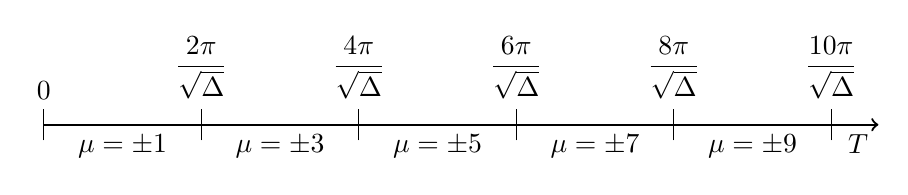
\begin{tikzpicture}
\draw[->,thick] (0,0)--(10.6,0) node[below left] {$T$};
\draw[] (0,-0.200)--(0,0.200) node[above] {0};
\foreach \i in {2,4,...,10}
\draw[] (\i,-0.200)--(\i,0.200) node[above] {$\displaystyle \frac{\i\pi}{\sqrt\Delta}$};


\foreach \i in {1,3,...,9}
\draw[] (\i,0) node[below] {$\mu = \pm \i$};
\end{tikzpicture}
\caption{Representation of the Conley-Zehnder index of the path $\exp(t J_0 S)$, $t \in \interval 0 T$ as a function of $T > 0$.}
\end{figure}
\end{itemize}
\end{prop}

\begin{proof}
We begin by solving the case $\Ind S = 1$. By inspection of equation \eqref{eq:exptj0s}, if $\Ind S = 1$ then both eigenvalues have distinct signs and $\det S = \Delta < 0$. Therefore, by \eqref{eq:exptj0s},
\begin{equation}
\trace \exp(t J_0 S) = 2 \cosh(\sqrt{-\Delta} t) \geq 2,
\end{equation}
where we used the trivially verified fact that $\trace(J_0 S) = 0$. Application of proposition \ref{calcmaslov} (to the extension of the path which ends in $W^-$) yields that, in this case, $\mu(x) = 0$.

We now focus on the case $\Ind S = 1 \pm 1$. In this case, by a similar calculation we obtain $\Delta > 0$ and furthermore
\begin{equation}
\trace \exp(t J_0 S) = 2 \cos(\sqrt\Delta t).
\end{equation}

Therefore, by corollary \ref{sp2sgn} the path $\exp(t J_0 S)$ is degenerate iff $\cos(\sqrt \Delta T) = 1$, which happens iff $\sqrt\Delta T \in 2 \pi \Z$. This completes the proof of nondegeneracy.

\smallskip

To compute the Maslov index, we apply proposition \ref{calcmaslov}.

There is an obstacle to the application of proposition \ref{calcmaslov}, which is that our path $A(t) = \exp(t J_0 S)$, $t \in \interval 0 T$, does not terminate at $W^\pm$. To rectify this, we work with the extension $\tilde A$, which consists of the path $A$ concatenated with a path from $A(T)$ to $W^\pm$. In the general case, this could cause us trouble because we might not know a lot about the extension, only that it exists. In this case, however, we can build this extension explicitly, in a manner that is convenient for computations.

In order to construct $\tilde A(t)$, suppose that $A(t)$ terminates at $t = T$, and let $T \in I_N$, where
\begin{equation}
I_N = \ointerval[scaled]{\frac{2\pi}{\sqrt\Delta} N}{\frac{2\pi}{\sqrt\Delta} (N+1)}.
\end{equation}

In the following, let $T' = \frac{2\pi}{\sqrt\Delta}(N+\frac12)$. There are two cases in the construction of $\tilde A(t)$. If $T \leq T'$, simply construct $\tilde A(t)$ by extending $A(t)$, with the same expression, to values of $t \in \interval 0 {T'}$. Otherwise, if $T > T'$, we extend $A(t)$ to $\tilde A(t)$ by `doubling back', setting $\tilde A(T+\delta) = A(T-\delta)$, for $0 < \delta < T-T'$.

In both cases, we have extended the path in such a way that the extension does not cross $Sp(2)^0$ any more than the original path $A(t)$ does, and the final value of $\tilde A(t)$ is, in both cases, $\exp(T J_0 S)$, which can be easily checked to equal $-I = W^+$. Therefore, the path $\tilde A(t)$ is in the conditions of proposition \ref{calcmaslov}, which we now apply.

First, we construct the partition. Let $T''$ be the terminating time of the path $\tilde A(t)$. Then, we consider the partition
\begin{equation}\label{autmaslov:thepartition}
\begin{array}{c|c|c|c|c|c|c|c|c}
a_0 & b_0 & a_1 & b_1
& \cdots &
b_{2N-1} & a_{2N} & b_{2N} & a_{2N+1} \\
\hline
0 & \frac12 \frac{\pi}{\sqrt\Delta} & \frac{\pi}{\sqrt\Delta} & \frac32 \frac{\pi}{\sqrt\Delta}
& \cdots &
\frac{2(2N-1)+1}2 \frac{\pi}{\sqrt\Delta} & 2N \frac{\pi}{\sqrt\Delta} & \frac{4N+1}2 \frac{\pi}{\sqrt\Delta} & T''
\end{array}
\end{equation}

It is necessary to verify that we are in the conditions of proposition \ref{calcmaslov}.
\begin{enumerate}
\item ($(-1)^n \trace \tilde A(a_n) \geq 2$) For $n \leq 2N$, we have that
\begin{equation}\label{eq:autmaslov1}
\trace \tilde A(a_n) = \trace A(a_n) = 2 \cos(\sqrt\Delta a_n) = 2 \cos\left(\sqrt\Delta \frac{n \pi}{\sqrt\Delta}\right) = 2 (-1)^n,
\end{equation}
so we have equality. For $n = 2N+1$, simply notice that $\tilde A(a_{2N+1}) = \tilde A(T'') = W^+$, which has trace equal to $-2$.

\item ($\trace \tilde A(b_n) = 0$) This property is a simple computation similar to \eqref{eq:autmaslov1}.

\item (Whenever $\trace \tilde A(x) \geq 2$ and $\trace \tilde A(y) \leq -2$, there exists some $b_n$ between $x$ and $y$.) To prove this property, simply notice that the points when the trace of $\tilde A(t)$ is equal to $\pm 2$ are known. Indeed, the trace is equal to $+2$ exactly on the points $t = a_0, a_2, \dots, a_{2N}$. Likewise, the trace is equal to $-2$ exactly on the points $t = a_1, a_3, \dots, a_{2N+1}$, and it is possible that there might be a point where $\tilde A(t)$ has trace 2 between $b_{2N}$ and $a_{2N+1}$. Given this study, the desired property is evident.
\end{enumerate}

Now that we have shown that partition \eqref{autmaslov:thepartition} satisfies the conditions necessary to apply proposition \ref{calcmaslov}, we simply apply it. This proposition tells us that the Maslov index of $\tilde A(t)$ is given by
\begin{equation}
\mu(\tilde A(t)) = \sum_{n = 0}^{2N} (-1)^n \sign(\tilde A(b_n)_{12}).
\end{equation}

Now, we may compute $\tilde A(b_n)$ explicitly as
\begin{equation}
\tilde A(b_n) = A(b_n) = \frac1{\sqrt\Delta} \sin\left( \sqrt\Delta \frac{2n + 1}2 \frac\pi{\sqrt\Delta} \right) J_0 S = (-1)^n J_0 S.
\end{equation}

Consequently, we have the identity
\begin{equation}
\mu(A(t)) = \mu(\tilde A(t)) = (2N+1) \sign((J_0 S)_{12}),
\end{equation}
and so it remains to relate the sign of $(J_0 S)_{12}$ to the index of $S$.

First, we make the trivial observation that $(J_0 S)_{12} = - S_{22}$, so we relate the sign of $S_{22}$ to the index of $S$.

Furthermore, observe that $S_{22}$ and $S_{11}$ have the same sign, as
\begin{equation}
S_{11} S_{22} = \Delta + S_{12}^2 > 0.
\end{equation}

Finally, this sign coincides with the sign of both eigenvalues of $S$ (which have the same sign because $\lambda_1 \lambda_2 = \Delta > 0$), and both of these signs equal the sign of the trace of $S$. In conclusion,
\begin{itemize}
\item The sign of $S_{22}$ equals the sign of the trace of $S$, which equals the sign of both eigenvalues of $S$.
\item Consequently, if $\Ind S = 0$ then these eigenvalues are positive, and therefore so is $S_{22}$ and therefore $(J_0 S)_{12} < 0$ and $\mu(A(t)) = -(2N+1)$.
\item On the other hand, if $\Ind S = 2$ then these eigenvalues are both negative, and by the same argument $\mu(A(t)) = 2N+1$.
\end{itemize}

The proof is therefore complete.
\end{proof}


